\documentclass{article}
\usepackage[utf8]{inputenc}
\usepackage{amsmath}
\usepackage{amsfonts}
\usepackage{amsthm}
\usepackage{graphicx}
\usepackage{setspace}
\usepackage{caption}
\usepackage{subcaption}
\usepackage{listings}
\usepackage{forest}
\usepackage{amsfonts}
\usepackage{array, makecell}
\usepackage{exercise}
\usepackage{kotex}
\usepackage{amssymb}
\usepackage{algorithm}
\usepackage{titlesec}   
\usepackage{algpseudocode}
\usepackage{fancyhdr}
\title{Discrete Mathematics Lecture Note}
\author{TaeYoung Rhee}
\date{October 2022}
\theoremstyle{definition}
\newtheorem{defn}{Definition}[]
\newtheorem{thm}{Theorem}[]
\newtheorem{ex}{Example}[]
\newtheorem{pp}{Proposition}
\newtheorem{nt}{Notation}
\newtheorem{cor}{Corollary}
\newtheorem{lm}{Lemma}
\newtheorem*{pf}{Proof}
\newenvironment{pf*}{\pushQED{\qed}\pf}{\popQED\endpf}
\setstretch{1.3}


\begin{document}

\maketitle

\section{Introduction}
\subsection{Mobius Inversion}
Let $D_n$ = all divisor set of positive integer $n$. \\
$a, b \in D_n, a \le b \Leftrightarrow a \vert b$  \\ 
Define $\mu : D_n \times  D_n \rightarrow \mathbb{R}$ 
\begin{align*}
    \mu(a,b) =
    \begin{cases}
        (-1)^r & \text{ if } a \;\vert\; b \text{ and } \frac{b}{a} 
        \text{ is the product of } k \text{ distinct primes} \\ 
        0 & \text{otherwise}
    \end{cases}
\end{align*}
\begin{align*}
    \mu (b) = \mu (1, b) = 
    \begin{cases}
        (-1)^r & \text{square free} \\ 
        0 & \text{not square free} 
    \end{cases}
\end{align*}
\begin{lm}
    For $m > 1$, 
    \begin{align*}
        \sum_{d \in D_m} \mu (d) =
        \begin{cases}
            1 & (m=1) \\ 
            0 & (m \ne 0) 
        \end{cases}
    \end{align*}
    \begin{align*}
        \sum_{a \le c \le b} \mu (a, c) = 
        \begin{cases}
            1 &  (a=b) \\ 
            0 & \text{otherwise}
        \end{cases}
    \end{align*}
    \begin{align*}
        \sum_{d} \mu (d) = \sum_{i=0}^{r} {r \choose i} (-1)^i = 0
    \end{align*}
\end{lm}
\begin{thm}
    For function $f, g : D_m \rightarrow \mathbb{R}$,
    \begin{align*}
        g(n) = \sum_{d\in D_n} f(d) \Leftrightarrow 
        f(n) = \sum_{d \in D_n} \mu (d, n) g(n) = \sum \mu (d) g(\frac{n}{d})
    \end{align*}
\end{thm}
\begin{pf*} $( \Rightarrow )$
    \begin{align*}
        &\sum_{d\in D_n} \mu (d, n) \sum_{e \in D_d} f(e) \\
        &= \sum_{e\in D_n} \sum_{e \le d \le d_n} \mu (d, n) f(e) \\ 
        &= \sum_{e \in D_n} f(e) \sum_{e \le d \le D_n} \mu (d, n) = f(n) 
    \end{align*}
\end{pf*}
\begin{cor}
    \begin{align*}
        \phi (n) = n \prod_{i=1}^{r} \left(1 - \frac{1}{p_i}\right) 
        \Leftrightarrow n = \sum_{d \in D_n} \phi (d)
    \end{align*}
    show that
    \begin{align*}
        \phi (n) = \sum_{d \in D_n} \mu (d) \frac{n}{d}
    \end{align*}
\end{cor}
\subsection{Generating Functions}
Define power series ring $\mathbb{C} [[x]] = \left\{ \sum_{n \ge 0} a_n x^n \vert 
a_n \in \mathbb{C}\; \forall n  \right\}$. `Formal' means evalutation or 
radius of convergence is ignored. We call $x^n$ is a `placeholder' of $a_n$.
$a_n$ = coefficient of $x^n$\\
For a sequence $f : N_0 \rightarrow \mathbb{C} \; \left(f \in \mathbb{C}[[x]]\right)$ \\ 
The ordinary generating function is 
\begin{align*}
    \sum f(n) x^n
\end{align*}
The exponential generating function is 
\begin{align*}
    \sum f(n) \frac{x^n}{n!}
\end{align*}
Let $A(x), B(x)$ ordinary. Then $AB = C$ is ordinary, where $c_n = 
\sum_{i=0}^n a_i b_{n-i}$ convolution. \\

Notation.
Define
$ e^x = \sum_{n\ge0} \frac{x^n}{n!}$ e.g.f for $(1,1,1, \cdots)$ \\ 
Define $e^{-x} = \sum_{n\ge0} (-1)^n \frac{x^n}{n!}$ \\ 
Show that $e^x e^{-x} = \left( \sum_{n\ge 0} \frac{x^n}{n!}\right)\left( \sum_{n\ge 0} (-1)^n  \frac{x^n}{n!}\right) = \sum_{n\ge 0} \left( \sum_{i=0}^n (-1)^i { n \choose i} \right) \frac{x^n}{n!}$ = 1. \\ 
Define $\log{1+x} = \sum_{n\ge 1} (-1)^{n-1} \frac{x^n}{n} $ \\ 
\begin{ex}
Generating function for $H_n = 1 + \frac{1}{2} + \cdots + \frac{1}{n}$ with $ H_0 = 0$ 
\begin{align*}
    &\sum_{n\ge 0} H_n x^n = \left( \sum_{n\ge 1} \frac{1}{n}x^n \right) \left( \sum_{n\ge 0 } x^n \right) \\
    & = -\log{(1-x)} \cdot (1-x)^{-1} \\ 
    & = \frac{1}{1-x}\log{\frac{1}{1-x}}
\end{align*}
\end{ex}
\subsection{Infinite Sums and Products in $\mathbb{C}[[x]]$}
\begin{ex}
$p(n) =$ $\#$ of partitions of $n$
\begin{align*}
    \sum_{n\ge 0 } p(n) x^n &= \prod_{i\ge 1} \frac{1}{1-x^i} \\ &= \frac{1}{1-x} \cdot \frac{1}{1-x^2} \cdots 
    \\ &= (1+x+x^2 +\cdots)(1+ x^2 + x^4 + \cdots) \cdots 
\end{align*}
Note that the coefficient of $x^n$ in 첫번째줄 requires finite number of factors. \\ 
\begin{align*}
    &\text{coefficient of } x^n \\ 
    &= \# \text{of solutions} (a_1, a_2, \cdots, a_n) 
    \text{ to } n_1 + 2n_2 + \cdots + = n \\ 
    &= p(n)
\end{align*}
\end{ex}
\begin{defn}
Let $A_0, A_1, \cdots \in \mathbb{C}[[x]]$ \\ 
$A \in \mathbb{C}[[x]]$, $\deg{(A)} = $ first power with nonzero coefficient. 
\end{defn}
The sum $\sum_{i\ge 0} A_i$ exists iff $\deg A_i \rightarrow \infty$.
\begin{align*}
    A_1 &= (a_{10}, a_{11}, a_{12}, a_{13}, \cdots) \\ 
    A_2 &= (0, a_{21}, a_{22}, a_{23}, \cdots) \\ 
    A_3 &= (9, 0, a_{32}, a_{33}, \cdots)
\end{align*}
We can make each row sum is finite.
\begin{ex}
    $e^{1+x}$ is not well-defined. 
    \begin{align*}
        e^{1+x} &= 1+ \left(1+x\right) + \frac{(1+x)^2}{2!} + \frac{(1+x)^3}{3!} + \cdots  
    \end{align*}
    \begin{align*}
        e^{e^x - 1} &= \sum_{n \ge 0} B(n) \frac{x^n}{n!} \\ 
        &= 1 + \left(\sum_{n\ge 1} \frac{x^n}{n!}\right) + \frac{\left(
            \sum_{n\ge 1} \frac{x^n}{n!}
        \right)^2}{2!} + \cdots
    \end{align*}
\end{ex} 
Assume the constant term of each $A_i =1$. 
$ \prod_{i\ge 1} A_i \text{ exists iff } \deg(A_i -1) \rightarrow \infty $
\begin{ex}
    $(1+x)(1+x^2)(1+x^3) \cdots $ is well defined.
    $= \sum_{n \ge 0} p_d(n) x^n$
\end{ex}

Propositions \\ 
(1) $\prod_{i\ge 0} A_i$ and $\prod_{i\ge 0 } B_i$ are well-defined $\Rightarrow \prod_{i\ge 0} A_i B_i = \left(\prod_{i\ge 0} A_i\right)\left(\prod_{i\ge 0} B_i\right)$
\begin{pf*}
    $\deg(AB - 1) \ge \min \{ \deg(A-1), \deg(B-1)\}$
    The factors that contribute to $x^n$ are the same on both sides
\end{pf*} 
(2) $\left( \prod_{i\ge 0} A_i  \right)^{-1} = \prod_{i\ge 0} A_i^{-1}$
\begin{pf*}
     dhotldqkfs
    \begin{align*}
        \deg(A_i - 1) = \deg(A_i^{-1} - 1)
    \end{align*}
    example \\ 
    \begin{align*}
        A = \prod_{i\ge 0} (i - x^{i}) \Rightarrow A^{-1} = \prod_{i\ge 0} \frac{1}{1-x^i}
    \end{align*}
\end{pf*}
(3) $ \frac{\prod_{i\ge 0 } A_i}{\prod_{i \ge 0} B_i} = \prod_{i\ge 0} \frac{A_i}{B_i}$
\begin{ex}
    $\frac{\prod_{i\ge 1}(1-x^{2i})}{\prod_{i\ge 1} (1-z^i)} = \prod_{i \ge 1} = \prod_{i\ge 1} (1+ z^i) = \sum_{n\ge 0} p_d(n) x^n
    = \prod_{i\ge 1} \frac{1}{1-z^{2i-1}} = \sum_{n\ge 0} p_0(n)x^n$ \\ 
    $p_0(n)$ is number of partitions of $n$ where parts are odd.
\end{ex}
\subsection{Compositions in $\mathbb{C}[[x]]$}
$A(x), B(x) \in \mathbb{C}[[x]]$ \\ 
$A(B(x))$ is well-defined if either (1) $A(x)$ is a polynomial or 
(2) the constant term in $B(x) = 0$
\begin{ex}
    \begin{align*}
        A(x) &= e^x \\ 
        B(x) &= e^x - 1
    \end{align*}
    $A(B(x)) = e^{e^{x} - 1}$. \\ 
    When $C(x) = x+1$, $A(C(x)) = e^{x+1}$ is not well defined.
\end{ex}
\subsection{General Powers}
Propositions. Given any $\lambda \in \mathbb{C}$, define 
${\lambda \choose n} = \frac{\lambda(\lambda-1)\cdots(\lambda-n+1)}{n!}$ with ${\lambda \choose 0} = 1$ \\ 
Define $(1+x)^{\lambda} = \sum_{n\ge 0} {\lambda \choose x^n} \in \mathbb{C}[[x]]$ \\ 
If $\lambda$ is a positive integer, this is just the binomial theorem. \\ 
If $A(x) \in \mathbb{C}[[x]]$ with $A(0) = 0$,
then $(1+ A(x))^\lambda = \sum_{n\ge 0} {\lambda \choose n} A(x)$.
\begin{ex}
    \begin{align*}
        (1-x)^{-k} \overset{?}{=} \frac{1}{(1-x)^k}
    \end{align*}
    Note that 
    \begin{align*}
        {-k \choose n} &= \frac{-k (-k -1)(-k -2 ) \cdots (-k-n+1)}{n!}\\ 
        &= \frac{(-1)^n (n+k-1)_n }{n!} \\ 
        &= (-1)^n {n + k - 1 \choose n} = (-1)^n { n+ k - 1\choose k - 1}
    \end{align*} 
    \begin{align*}
        (1-x)^{-k} &= \sum_{n\ge 0} {-k \choose n} (-1)^n x^n \\ 
        &= \sum_{n \ge 0} {n+k -1 \choose k -1} x^n = \frac{1}{(1-x)^k}
    \end{align*}
\end{ex}
Proposition. $(1+x)^\lambda (1+x)^\mu = (1+x)^{\lambda + \mu}$
\begin{ex}
    \begin{align*}
        (1+x)^{\frac{1}{2}} ( 1+ x)^{\frac{1}{2}} = 1 + x
    \end{align*}
\end{ex}
\begin{pf*}
    Need to show 
    \begin{align*}
        \sum_{i=0}^n {\lambda \choose i} {\mu \choose n-i} = 
        {\lambda + \mu \choose \mu} \text{ for all } n \ge 0 
    \end{align*}
    We can prove it in algebra. 
    Otherwise, we can show it by proving coefficient of $x^n$ for LHS $=$ 
    coefficient of $x^n$ for RHS.\\ 
    Check that 
    \begin{align*}
        {x+y \choose n} = \sum_{i=0}^n { x \choose i}{y \choose n - i}
        \text{ for all positive integers } x, y
    \end{align*}
    Let LHS = $f(x, y)$ and RHS = $g(x,y)$. \\ 
    $f(x, y) = g(x, y)$ for infinitely many $x, y$ \\ 
    $f=g$ as polynomials.
\end{pf*} 

\subsection{Catalan Numbers}
\begin{align*}
    &c_0 = 0, c_1 = 1, c_2 = 1, c_3 = 2, c_4 = 5 \\ 
    &c_5 = c_1 c_4 + c_2 c_3 + c_3 c_3 + c_4c_1 \\ 
\end{align*}
\begin{align*}
    c_n = \sum_{i=1}^{n-1} c_i c_{n-i}
\end{align*}
Let $C(x) = \sum_{n\ge 0} c_n x^n$. 
\begin{align*}
    &C(x) = C(x)^2 + x \\ 
    & \Rightarrow C(x)^2 - C(x) = -x \\ 
    & \Rightarrow C(x)^2 - C(x) + \frac{1}{4} = \frac{1}{4} - x\\
    & \Rightarrow \left(C(x) - \frac{1}{2}\right)^2 = \frac{1}{4} - x\\
    & \Rightarrow C(x) - \frac{1}{2} = \pm \frac{1}{2} (1-4x)^{\frac{1}{2}}
\end{align*}
Since $C(x) = c_0 = 0$, we get 
\begin{align*}
    &C(x) - \frac{1}{2} = -\frac{1}{2}(1-4x)^{\frac{1}{2}} \\ 
    &\therefore C(x) = \frac{1}{2} -  \frac{1}{2}(1-4x)^{\frac{1}{2}}
\end{align*}
\begin{align*}
    (1-4x)^{\frac{1}{2}} &= 1 + \sum_{n\ge 1} {\frac{1}{2} \choose n} (-1)^n 4^n x^n \\ 
    &= 1- 2\sum_{n\ge 1}\frac{1}{n}{2n-2 \choose n-1 } x^n
\end{align*}
Check that 
\begin{align*}
    {1\frac{1}{2} \choose n} = \frac{(-1)^{n-1}}{2^{2n-1}}\frac{1}{n}{2n -2 \choose n-1}
\end{align*}
Thus
\begin{align*}
    c_n = \frac{1}{n} {2n-2\choose n-1}
\end{align*}
\subsection{Other interpretations of Catalan Number}
$c_n =$ number of ways to parenthesize a product $x_1 x_2 \cdots x_n$  
\begin{ex}
    For $x_1 x_2 x_3 x_4$, there are 5 ways. \\ 
    Key observation is the outermost parenthesis multiples two terms.
    The first is a product involving $x_1, x_2, \cdots , x_r$ $\rightarrow$ $a_r$ 
    ways to do this. The second is a product involving $x_r+1, x_r+2, \cdots, x_n$ $\rightarrow$
    $a_{n-r}$ ways.
\end{ex}
number of binary trees with $n$ leaves and 1 root. A tree is binary if 
every vertex has degree 1 or 3. \\ 
\begin{figure}[!h]
    \centerline{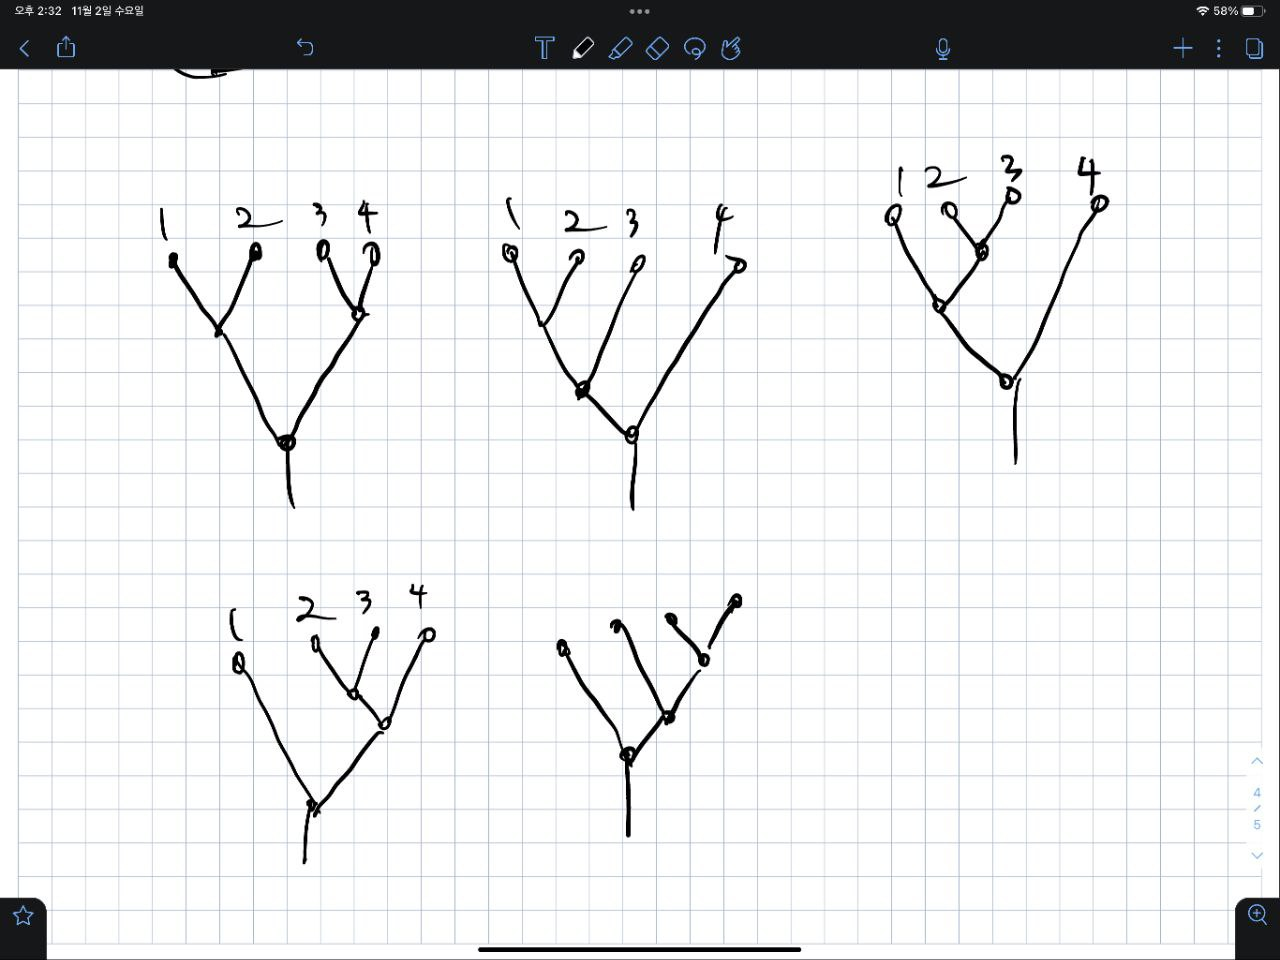
\includegraphics[width=0.5\columnwidth]{tree.jpg}}
    \caption{binary tree}
    \label{tree} 
\end{figure}
A bijections among these sets (triangulations of $n+1$-gon, parenthesized products
of $n$ vatiables, binary trees with $n$ leaves)
\begin{ex}
    Figure \ref{figure_1} is the bijection between the sets.
    \begin{figure}[!h]
        \centerline{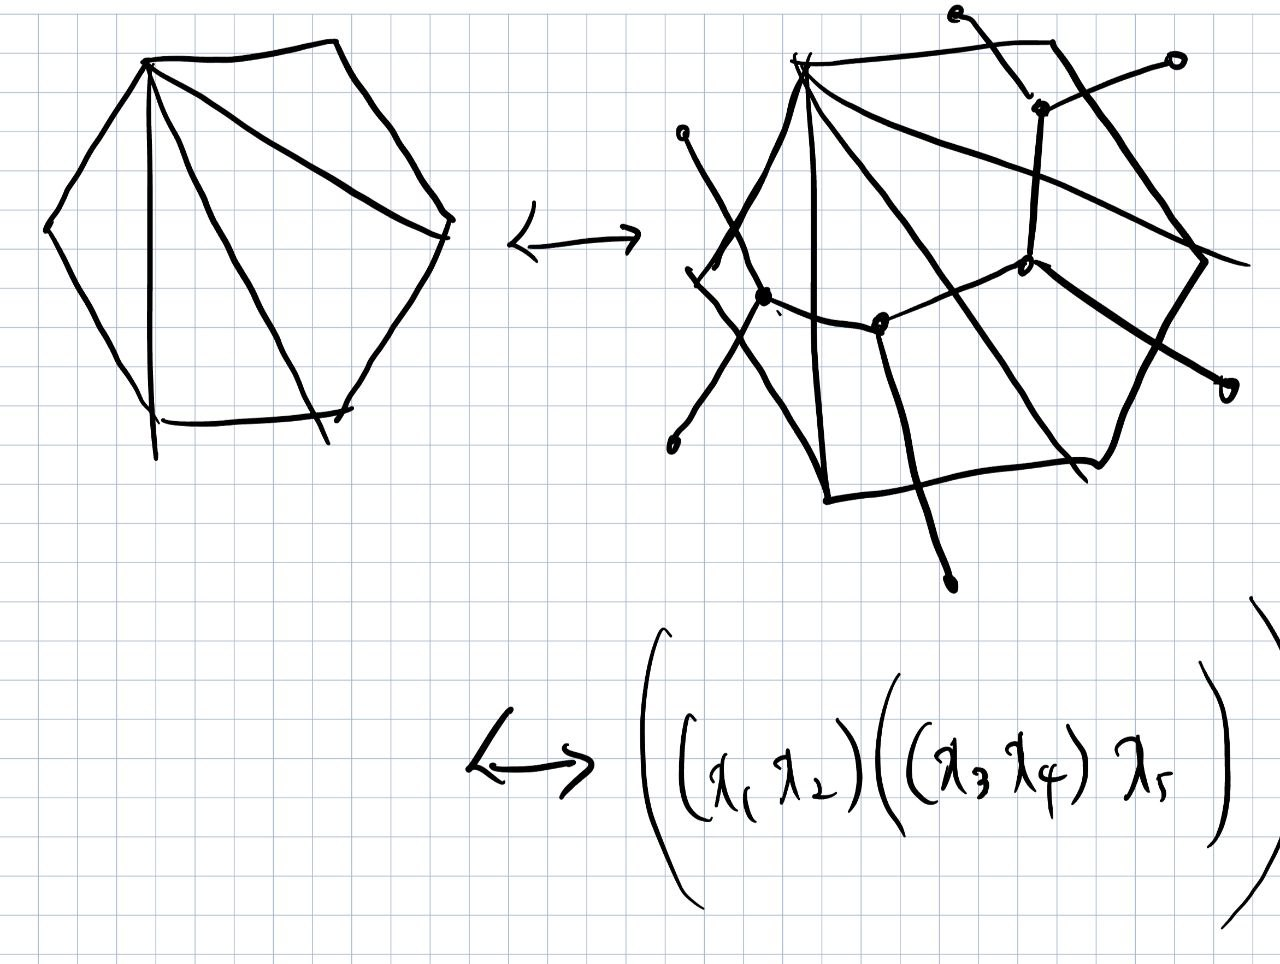
\includegraphics[width=0.5\columnwidth]{bijection_gon.jpg}}
        \caption{bijections}
        \label{figure_1} 
    \end{figure}
\end{ex}
\subsection{Product of exponential generating functions}
\begin{align*}
    A(x) &= \sum_{n\ge 0} a_n \frac{x^n}{n!} \\ 
    B(x) &= \sum_{n\ge 0} b_n \frac{x^n}{n!}
\end{align*}
\begin{align*}
    A(x)B(x) = \sum_{n\ge 0} c_n \frac{x^n}{n!} \text{ where } 
    c_n = \sum_{i=0}^{n} {n \choose i} a_i b_{n-i}
\end{align*}
It means number of ways to partition on $n$-set into 
two ordered blocks and create structure ``$A$'' in the 
first block and structure ``$B$'' in the second block. \\ 
\textbf{Remark} If ``$A$'' = ``$B$'', then $\frac{A(x)^2}{2!} = $ e.g.f
for the number of ways to create two unordered blocks in an $n$-set and create
structure ``$A$'' in each block.\\ 
\textbf{Remark} If both blocks of an $n$-set has to be non-empty then
let $a_0=b_0=0$ 
\begin{ex}
    $c_n = $ number of ways to color $n$ labeled balls with red and blue
    so that an even number of balls are colored red and an odd number of balls
    are colored blue.\\ 
    $c_n = 0$ if $n$ is even. $c_n = 2^{n-1}$ if $n$ is odd.\\
    $R(x) = $ e.g.f for $(1,0,1,0,\cdots) = 1 + \frac{x^2}{2!} + \frac{x^4}{4!} = 
    \frac{e^x + e^{-x}}{2}$\\ 
    $B(x) = $ e.g.f for 
    $(0,1,0,1,\cdots) = x + \frac{x^3}{3!} + \frac{x^5}{5!} + \cdots = 
    \frac{e^x - e^{-x}}{2}$
    \begin{align*}
        \sum_{n\ge 0} c_n \frac{x^n}{n!} &= C(x) = R(x)\cdot B(x) \\ 
        &= \frac{e^{2x} - e^{-2x}}{4} \\ 
        &= \frac{1}{4} \left[\left(1 + 2x + \frac{(2x)^2}{2!} + \cdots \right) - 
        \left(1 - 2x + \frac{(2x)^2}{2!} - \cdots \right)\right]\\ 
        &= \sum_{n\ge 0 \; n \text{ odd}} 2^{n-1} \frac{x^n}{n!}
    \end{align*}
\end{ex}
\begin{ex}
    Dearangement (revisited) 
    \begin{align*}
        P(x) = \sum_{n \ge 0} n! \frac{x^n}{n!} = \sum_{n \ge 0} x^n 
        = \frac{1}{1-x} = \text{ e.g.f for } \{ \vert S_n \vert = n! \} 
    \end{align*}
    \begin{align*}
        I(X) &= \sum_{n\ge 0} 1 \frac{x^n}{n!} = e^x \\ 
        & = \text{ e.g.f for the number of identity permutations on an } n \text{-set} \\ 
        & = \text{ e.g.f for the sequence } (1, 1, 1, \cdots )
    \end{align*}
    \begin{align*}
        D(x) = \sum_{n\ge 0} d_n \frac{x^n}{n!} \text{ where } d_n= 
        \text{ number of dearangements on an } n \text{-set}
    \end{align*}
    $P(x) = I(x)D(x)$ because a permutations on an $n$-set is obtained by 
    \begin{enumerate}
        \item partitioning the $n$-set into two ordered blocks.
        \item create the identity permutations on the first block and
        create a dearangement on the second block.
    \end{enumerate}
    \begin{align*}
        \therefore D(x) = P(x)I(x)^{-1} = \frac{e^{-x}}{1-x}
    \end{align*}
\end{ex}
\subsection*{PS3 \#7}
number of involutions in $S_n$ = number of partial matchings with $n$ verticies
= $a_n$ \\ 
partial matching = degree $1$ graphs = collection of disjoint edges and vertices. \\ 
$\sigma \in S_n$ is an involution if $\sigma = id$, i.e., $\sigma$ is a
product of disjoint transpositions cycles of length 2. \\ 
partial matchings is 
\begin{enumerate}
    \item Split $[n]$ into two blocks.
    \item Create a perfect matching in the first block and leave
    the second block untouched.
\end{enumerate}
For PS3 \#7 (a), check that $a_n = a_{n-1} + (n-1) a_{n-2}$ 
with $a_0 = a_1 =1$. \\ 
(b) 
\begin{align*}
    f(x) = \sum_{n\ge 0} a_n \frac{x^n}{n!} &= e^{x + \frac{x^2}{2}} \\
    &= 1 + (x + \frac{x^2}{2}) + \frac{\left(x+\frac{x^2}{2}\right)}{2!} + \cdots \\ 
    &= 1+ x + \sum_{n\ge 2} (a_{n-1} + (n-1)a_{n-2}) \frac{x^n}{n!}
\end{align*}
\begin{align*}
    f'(x) &= 1 + \sum_{n\ge 2} a_{n-1} \frac{x^{n-1}}{(n-1)!} 
    + \sum_{n \ge 2} a_{n-2} \frac{x^{n-1}}{(n-2)!} \\ 
    &= 1 + (f(x) - 1) + xf(x) \\
    &\Rightarrow f'(x) = (1+x)f(x) \\ 
    &\Rightarrow \frac{f'(x)}{f(x)} = 1 + x \\ 
    &\Rightarrow f(x) = e^{x + \frac{x^2}{2}}
\end{align*}
Let $g(x) = e^{x + \frac{x^2}{2}} = \sum_{n\ge 0} b_n \frac{x^n}{n!}$. \\ 
Since $g'(x) = (1+x) g(x)$. \\ 
We can check that $b_n = b_{n-1} + (n-1)b_{n-2}$ with $b_0 = b_1 = 1$. \\
Then $\{a_n\}$ and $\{b_n\}$ satisfies the same recurrance relations 
\begin{align*}
    \therefore  \forall n \;\; a_n = b_n
\end{align*}
Review: $S(n,k)$ = Stirling numbers of the second kind. \\ 
$k!S(n,k)$ = number of all surjective functions $f: [n] \rightarrow k$ ($k$ fixed)\\ 
= $\sum_{(n_1, n_2, \cdots , n_k)} {n \choose n_1, n_2, \cdots, n_k}$ where
the sum is over all compositions $(n_1, \cdots, n_k)$ of $n$.
\begin{align*}
    \Rightarrow S(n,k) &= \frac{1}{k!} \sum_{(n_1, \cdots, n_k)} {n \choose 
    n_1, n_2, \cdots, n_k} \\
    &= \frac{1}{k!} \times \left(\text{coefficient of } \frac{x^n}{n!} 
    \text{ in } (e^x - 1)^k\right) \\ 
    &= \frac{1}{k!} \sum_{(n_1, \cdots, n_k)} {n \choose n_1, n_2, \cdots, n_k}
    \overbrace{1 \cdot 1 \cdots 1}^{k \text{ times }}
\end{align*}
\begin{align*}
    \sum_{n\ge 0} S(n,k) \frac{x^n}{n!} = \frac{(e^x - 1)^k}{k!} 
\end{align*}
\begin{cor}
    \begin{align*}
        f_n &= \text{ number of surjections } [n] \rightarrow [k] \\ 
        &\sum_{n \ge 0}f_n \frac{x^n}{n!} = (e^x - 1)^k
    \end{align*}
\end{cor}
Exercise. Let $g_n =$ number of surjections with $\vert f^{-1}(i)\vert \ge 3 
\; \forall i \in [k]$. Find $sum_{n\ge 0} g_n \frac{x^n}{n!}$.
\begin{pp}
    Let $A(x) = \sum_{n\ge 0} a_n \frac{x^n}{n!}$ where $a_n$ = number of
    ways to create structure ``$A$'' on an $n$-set. \\ 
    Then 
    \begin{align*}
        \frac{A(x)^k}{k!} = \sum_{n\ge 0} b_n \frac{x^n}{n!}
    \end{align*}
    where $b_n$ = number of ways to 
    \begin{enumerate}
        \item partition an $n$-set into unordered $k$ blocks 
        \item create structure ``$A$'' in each block.
    \end{enumerate}
\end{pp}
\begin{proof}
    clear.
\end{proof}
\begin{ex}
    $c(n,k)$ = number of ways to create $k$ cycles on $[n]$. \\ 
    Let $A(x) = \sum_{n\ge 1} (n-1)! \frac{x^n}{n!} = \sum_{n\ge 1} 
    \frac{x^n}{n} = - \log (1-x) = \log(\frac{1}{1-x})$. \\
    $(n-1)!$ is the number of ways to create one cycle of length $n$
    \begin{align*}
        \therefore \sum_{n\ge 0} c(n,k)\frac{x^n}{n!} 
        = \frac{\log\left(\frac{1}{1-x}\right)^k}{k!}
    \end{align*}
\end{ex}
\begin{thm}
    Let $A(x) = \sum_{n \ge 1} a_n \frac{x^n}{n!} \; (n \ge 1)$
    \begin{align*}
        e^{A(x)} = \exp \left(\sum_{n\ge 1} a_n \frac{x^n}{n!}\right) 
        = \sum_{n \ge 0} b_n \frac{x^n}{n!} \; (b_0 = 1)
    \end{align*}
    where $b_n$ = number of ways to partition an $n$-set into unordered
    non-empty blocks and create structure ``$A$'' in each block.
\end{thm}
\begin{pf*}
    \begin{align*}
        e^{A(x)} = 1 + A(x) + \frac{A(x)^2}{2!} + \cdots + \frac{A(x)^k}{k!} + \cdots
    \end{align*}
    coefficient of $\frac{x^n}{n!}$ in $e^{A(x)}$ = $\sum_{k\ge 1} 
    \text{ coefficient of } \frac{x^n}{n!} \text{ in } \frac{A(x)^k}{k!}$
    \\ which means the number of ways to partition an 
    $n$-set into unordered
    non-empty blocks and create structure ``$A$'' in each block.
\end{pf*}
\begin{ex}
    \begin{align*}
        \sum_{n\ge 0} B(n) \frac{x^n}{n!}
        &= \sum_{n \ge 0} \left(\sum_{k \ge 0} S(n, k)\right)\frac{x^n}{n!} \\ 
        &= \sum_{k \ge 0} \left( \sum_{n \ge 0} S(n,k) \frac{x^n}{n!}\right) \\ 
        &= \sum_{k \ge 0} \frac{(e^x -1)^k}{k!} = e^{e^x - 1}
    \end{align*}
    where $B(n)$ is Bell number. 
\end{ex}
\begin{ex}
    \begin{align*}
        A(x) = \sum_{n\ge 1} \frac{x^n}{n!} = \log \left(\frac{1}{1-x}\right)
    \end{align*}
    \begin{align*}
        \frac{1}{1-x } &= \sum n! \frac{x^n}{n!} \\ 
        &= \sum_{n\ge 0} \vert S_n \vert \frac{x^n}{n!} \\ 
        &= e^{A(x)} = e^{\log \left(\frac{1}{1-x}\right)} = \frac{1}{1-x}
    \end{align*}
\end{ex}
\begin{ex}
    number of simple graphs on the vertext set $[n]$ = $2^{n \choose 2}$. Simple
    graph is a compound structure given by connected graphs. \\ 
    graph figre\\ 
    Let $f(x) = \sum_{n\ge 1} d_n \frac{x^n}{n!}$ where $d_n = $ number of
    connected graphs on an $n$-vertext set. \\
    We know that $2^{n \choose 2}$ = number of simple graphs on $n$-vertices.
    \begin{align*}
        e^{f(x)} &= \sum_{n\ge 0} 2^{{n \choose 2}} \frac{x^n}{n!} \; 
        \left({0 \choose 2} = {1 \choose 2} = 0\right) \\ 
        f(x) &= \log \left( \sum_{n\ge 0} 2^{{n \choose 2}} \frac{x^n}{n!} \right) \\ 
        \overset{diff}{\Rightarrow} f'(x) = \frac{\text{aaa}'}{\text{aaa} }
    \end{align*}  
    \begin{align*}
        \left(\sum_{n\ge 1} n d_n \frac{x^{n-1}}{n!}\right) \left(
            \sum_{n\ge 0} 2^{n \choose 2} \frac{x^{n-1}}{n!} 
        \right) = \sum_{n\ge 0} n 2^{n \choose 2} \frac{x^n}{n!}
    \end{align*}
    By comparing the coefficient of $\frac{x^n}{n!}$ on both sides.
    \begin{align*}
        \sum_{i=1}^n {n \choose i} i \cdot d_i 2^{n-i \choose 2} = n 2^{n \choose 2}
    \end{align*}
    \begin{align*}
        &n = 1 : d_1 = 1 \\
        &n =2  : {2 \choose 1} d_1 + {2 \choose 2} d_2 = 2 \cdot 2 \\ 
        &\Rightarrow d_2 = 1, d_3 = 4
    \end{align*}
\end{ex}
\begin{defn}
    Tree = a connected acyclic group
\end{defn}
Cayley: number of spanning trees in $K_n = n^{n-2}$
\begin{ex}
    $n=3: 3^1 =3$ \\ 
    3 spanning tree grim \\ 
    $n = 4: 4^2 = 16$ \\ 
    4 spanning tree grim 
\end{ex}
\begin{defn}
    Forest = a disjoint union of trees
\end{defn}
\begin{ex}
    For $n=3$, \\ 
    forest grim
\end{ex}
Define tree generating function. 
\begin{align*}
    T(x) = \sum_{n \ge 1} n^{n-2} \frac{x^n}{n!} 
\end{align*}
\begin{align*}
    e^{T(x)} = \sum_{n\ge 0} r_n \frac{x^n}{n!} 
\end{align*}
where $r_n$ is the number of spanning forests in $K_n$
\begin{align*}
    e^{T(x)} = 1 + T(x) + \frac{T(x)^2}{2!} + \cdots
\end{align*}
We can think coefficient of $\frac{x^n}{n!}$ in $\frac{T(x)^k}{k!} \; (k\ge 0)$ \\ 
coef pyo \\ 
Define $f$-vector of $K_n$ 
\begin{align*}
    f_{K_n} &= (f_0, f_1, \cdots , f_{n-1}) \\ 
    f_{K_4} &= (1, 6, 15, 16) \;\; (15^2 \ge 6 \cdot 16)\\ 
    f_{K_5} &= (1, 10, 45, 110, 123)  \;\; (45^2 \ge 10 \cdot 110)\\ 
    f_{K_6} &= (1, 15, 105, 435, 1080, 1296)
\end{align*}
Log-cocavity of $f_{K_n}$ (proved by Heo) \\ 
Define an alternating sum 
\begin{align*}
    \alpha (K_n) = f_{n-1} - f_{n-2} + f_{n-3} - \cdots \pm f_0
\end{align*}
\begin{center}
    \begin{tabular}{c|ccccc}
        $n$ & 2 & 3 & 4 & 5 & 6 \\ 
        \hline 
        $\alpha(K_n)$ & 0 & 1 & 6 & 61 & 560
    \end{tabular}
\end{center}
\begin{align*}
    -e^{-T(x)} = 1 - T(x) + \frac{T(x)^2}{2!} - \cdots = \sum_{n\ge 0} 
    \alpha (K_n) \frac{x^n}{n!}
\end{align*}
\subsection{Generating Functions for Number Partitons}
We know $p(n) =$ number of partitons $\lambda = \lambda_1 \ge \lambda_2 
\ge \cdots$ of $n$ 
= number of weak solutions to $a_1 + 2a_2 +3a_3 + \cdots + n a_n = n$
\begin{thm}
    \begin{align*}
        \sum_{n \ge 0} p(n) x^n = \prod_{i \ge 1} \frac{1}{1-x^i} 
    \end{align*}
\end{thm}
\begin{pf*}
    \begin{align*}
        \prod_{i\ge 1} \frac{1}{1-x^i} &= \frac{1}{1-x} \cdot \frac{1}{1-x^2} \cdots \\ 
        &= (1+x+x^2+\cdots ) (1+ x^2 +x^4 + \cdots ) \cdots 
    \end{align*}
    coefficient of $x^n$ = number of sequence $(a_1, a_2, \cdots, a_n)$ 
    satisfying $a_1 + 2a_2 + \cdots + na_n = n$ is $p(n)$
\end{pf*}
$p_d (n)$ = number of partitions of $n$ with distinct part.
\begin{align*}
    \sum_{n\ge 0} p_d (n) x^n = \prod_{i \ge 1} (1+ x^i)
\end{align*}
$p_o (n)$ = number of partitions of $n$ with parts that are odd only. 
\begin{align*}
    \sum_{n \ge 0} p_o (n) x^n = \prod{i \ge 1} \frac{1}{1- x^{2i - 1}}
\end{align*}
Euler. $p_d (n) = p_o (n)$
\begin{pf*}
    \begin{align*}
        \prod_{i\ge 1 } (1+x^i) &= (1+x) (1+ x^2) ( 1+ x^3) \cdots \\ 
        &= \frac{1-x^2}{1-x} \frac{1-x^4}{1-x^2} \frac{1-x^6}{1-x^3} \cdots \\ 
        &= \prod_{i\ge 1} \frac{1}{1-x^{2i-1}} 
    \end{align*}
\end{pf*}
Combinatirocial proof of $p_d (n) = p_o (n)$
\begin{lm}
    $t_n$ = number of partitions of $n$ into distinct powers of 2 = 1 $\forall n$
\end{lm}
\begin{pf*}
    \begin{align*}
        (1+x) (1+x^2) (1+x^4) (1+x^8) \cdots = 1 + x + x^2 + \cdots 
    \end{align*}
\end{pf*}
\begin{ex}
    \begin{align*}
        \lambda &= ( 12 , 9, 7, 6, 3, 2) \in {Par}_d (39) \\ 
        12 &= 2^2 \cdot 3 \\ 
        9 &= 2^0 \cdot 9 \\ 
        7 &= 2^0 \cdot 7 \\ 
        6 &= 2^1 \cdot 3 \\
        3 &= 2^0 \cdot 3 \\ 
        2 &= 2^1 \cdot 1
    \end{align*}
\end{ex}
We can get $\overset{\sim}{\lambda} = ( 9, 7, 3, 3, 3, 3, 3, 3, 3, 1, 1)$. 
We know how many 3 used and decompose $7 = 2^2 + 2^1 + 2^0$. 
\begin{ex}
    number of $\lambda \vdash n$ s.t. only odd parts may be repeated 
    = number of $\lambda \vdash n$ s.t. no part appears more than 3 times.
\end{ex}
The generating function of first part is 
\begin{align*}
    &\frac{1}{1-x} (1+x^2) \frac{1}{1-x^3} (1+x^4) \cdots  \\ 
    &= \frac{1}{1-x} \frac{(1+x^2)(1-x^2)}{1-x^2} \frac{1}{1-x^2} 
    \frac{(1+x^4)(1-x^4)}{(1-x^4)} \cdots \\
    &= \frac{1}{1-x} \frac{(1-x^4)}{1-x^2} \frac{1}{1-x^2} 
    \frac{(1-x^8)}{(1-x^4)} \cdots \\ 
    &= (1+x + x^2 + x^3)(1+ x^2 +x^4 +x^6) \cdots 
\end{align*}
\end{document}  